\documentclass[10pt]{article}

\usepackage[margin=0.75in]{geometry}
\usepackage{amsmath,amsthm,amssymb}
\usepackage{xcolor}
\usepackage{cancel}
\usepackage{graphicx}
\usepackage{changepage}
\usepackage{circuitikz}
\usepackage{pgfplots}
\usepackage{physics}
\usepackage{hyperref}
\usepackage{siunitx}
\usepackage{fontspec}
\usepackage{relsize}
\usepackage{subfig}
\usepackage{todonotes}
\usepackage{minted}
\usepackage{multicol, multirow, booktabs}
\usepackage[breakable]{tcolorbox}
\usepackage[inline]{enumitem}

\theoremstyle{definition}
\newtheorem{problem}{Problem}
\newtheorem{soln}{Solution}

\pgfplotsset{compat=newest}
\usetikzlibrary{lindenmayersystems}
\usetikzlibrary{arrows}
\usetikzlibrary{calc}
\usetikzlibrary{positioning, fit}
\usetikzlibrary{3d, perspective}

\definecolor{incolor}{HTML}{303F9F}
\definecolor{outcolor}{HTML}{D84315}
\definecolor{cellborder}{HTML}{CFCFCF}
\definecolor{cellbackground}{HTML}{F7F7F7}
\newcommand{\ui}{\hat{i}}
\newcommand{\uj}{\hat{j}}
\newcommand{\uk}{\hat{k}}
\newcommand{\ux}{\hat{x}}
\newcommand{\uy}{\hat{y}}
\newcommand{\uz}{\hat{z}}
\newcommand{\primed}[1]{#1^\prime}
\pgfdeclarelayer{background}  
\pgfsetlayers{background,main}
\AtBeginDocument{\RenewCommandCopy\qty\SI}

\makeatletter
\newcommand{\boxspacing}{\kern\kvtcb@left@rule\kern\kvtcb@boxsep}
\makeatother
\newcommand{\prompt}[4]{
    \ttfamily\llap{{\color{#2}[#3]:\hspace{3pt}#4}}\vspace{-\baselineskip}
}

\newcommand{\thevenin}[2]{
  \begin{center}
    \begin{circuitikz} \draw
      (0,0) -- (2,0) to[battery1, l_=$V_{Th}\eq#1$] (2,2) 
      to[resistor, l_=$R_{Th}\eq#2$] (0,2)
      ;
      \draw [o-] (-.07,2.079);
      \draw [o-] (-.07,0.079);
    \end{circuitikz}
  \end{center}
}

\newcommand{\norton}[2]{
  \begin{center}
    \begin{circuitikz} \draw
      (0,0) -- (3,0) to[american current source, l_=$I_{N}\eq#1$] (3,2) -- (0,2) (2,0)
      to[resistor, l=$R_{N}\eq#2$] (2,2)
      ;
      \draw [o-] (-.07,2.079);
      \draw [o-] (-.07,0.079);
    \end{circuitikz}
  \end{center}
}

\newcommand{\highlight}[1]{\colorbox{yellow}{$\displaystyle #1$}}

\newcommand{\ti}[1]{\widetilde{#1}}

\newfontface{\Kaufmann}{Kaufmann}
\DeclareTextFontCommand{\kf}{\Kaufmann}
\newcommand{\scriptr}{\fontsize{12pt}{12pt}\kf{r}}

\newfontface{\KaufmannB}{Kaufmann Bd BT}
\DeclareTextFontCommand{\kfb}{\KaufmannB}
\newcommand{\bscriptr}{\fontsize{12pt}{12pt}\kfb{r}}

\newcommand{\bv}[1]{\mathbf{#1}}

\title{Physics 3610H: Assignment III}
\author{Jeremy Favro (0805980) \\ Trent University, Peterborough, ON, Canada}
\date{\today}

\begin{document}
\maketitle

% PROBLEM 1
\begin{problem}
Consider a particle in the infinite square well from $0<x<a$. The eigenstates and eigenvalues of the
T.D.S.E for this system are
\begin{align*}
  \psi_n(x) & =\sqrt{\frac{2}{a}}\sin\left(\frac{n\pi x}{a}\right) \\
  E_n       & =\frac{\hbar^2n^2\pi^2}{2ma^2}
\end{align*}
respectively. We also found that these states form an orthonormal set,
$$
  \int_{\mathbb{R}}\psi^*_n(x)\psi_m(x)dx=\delta_{mn}.
$$
Suppose a particle in such a well is in the following state at $t=0$:
$$
  \Psi(x,0)=A(\psi_1(x)+2\psi_2(x))
$$
\begin{enumerate}[label=(\alph*)]
  \item Find $A$ such that $\Psi(x,0)$ is normalized.
  \item Draw $\Psi(x,0)$ as a function of $x$.
  \item Where is the particle most likely to be found at $t = 0$? (Draw arrow(s) on your plot.)
  \item Where is the particle least likely to be found at $t = 0$? (Draw arrow(s) on your plot.)
  \item What is the probability of finding the particle in the left half of the well (i.e. $0 < x < a/2$)
        at $t = 0$?
  \item Find $\Psi(x,t)$.
  \item Show $\Psi(x,t)$ is normalized for all times $t$.
  \item What is the expectation value of $x$?
  \item If you measured the energy of this particle, what values might you get and what is the
        probability that you will get each of these values?
  \item What is the expectation value of the energy?
\end{enumerate}
\end{problem}
\newpage
\begin{soln}~
  \begin{enumerate}[label=(\alph*)]
    \item Here we force the integral over all space of $\abs{\Psi}^2$ to be 1 and solve for an $A$ which satisfies this. We can note
          that because we are dealing with an infinite well here the wavefunction is only nonzero within the well so we can trim down the bounds a bit,
          \begin{align*}
            1 & =\int_{0}^{a}\Psi^*(x,0)\Psi(x,0)\,dx                                                                            \\
              & =\abs{A}^2\int_{0}^{a}(\psi_1^*(x)+2\psi_2^*(x))(\psi_1(x)+2\psi_2(x))\,dx                                       \\
              & =\abs{A}^2\int_{0}^{a}\psi_1^*(x)\psi_1(x)+2\psi_2^*(x)\psi_1(x)+2\psi_2(x)\psi_1^*(x)+4\psi_2(x)\psi_2^*(x)\,dx \\
              & =\abs{A}^2\int_{0}^{a}\psi_1^*(x)\psi_1(x)+2\delta_{12}+2\delta_{12}+4\psi_2(x)\psi_2^*(x)\,dx                   \\
              & =\abs{A}^2\left[\delta_{11}+\cancelto{0}{\delta_{12}+\delta_{12}}+4\delta_{22}\right]                            \\
              & =\abs{A}^2\left[1+4\right]\implies \abs{A}^2=1/5\implies A=\sqrt{1/5}
          \end{align*}
    \item ~\\
          \begin{center}
            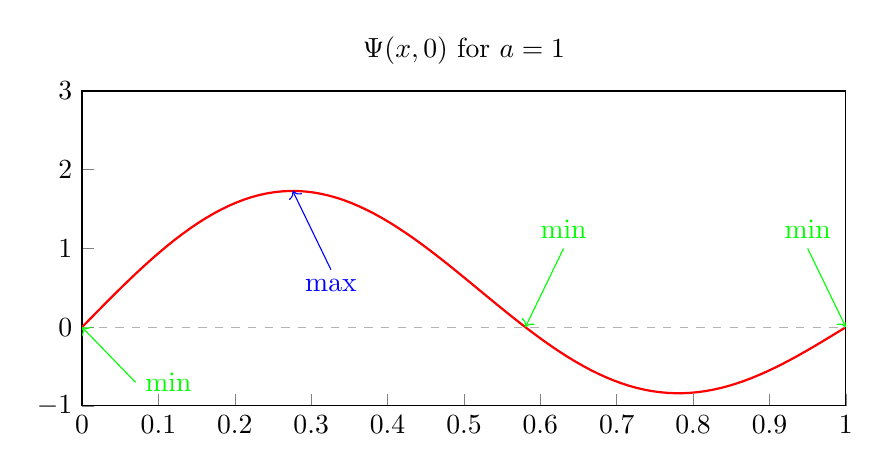
\begin{tikzpicture}
              \begin{axis}[title = {$\Psi(x,0)$ for $a=1$},
                  ymax = 3,
                  ymin = -1,
                  xmin=0,
                  xmax=1,
                  xtick pos = bottom,
                  ytick pos = left,
                  height=4cm,
                  width=0.8\textwidth,
                  scale only axis=true]
                \draw[red, thick, domain=0:1, samples=100] plot (\x, {
                    sqrt(1/5)*(sqrt(2)*sin(deg(pi*\x))+2*sqrt(2)*sin(deg(2*pi*\x)))
                  });
                \draw[black!30, dashed, domain=0:1, samples=1] plot (\x,0);
                \coordinate (MAX) at (0.27587156664462037, {sqrt(1/5)*(sqrt(2)*sin(deg(pi*0.27587156664462037))+2*sqrt(2)*sin(deg(2*pi*0.27587156664462037)))});
                \draw[blue, <-] (MAX) -- +(+0.05, -2) node[below]{max};

                \draw[green, <-] (0.5804306232551663, 0) -- +(+0.05, 0) node[above]{min};
                \draw[green, <-] (0, 0) -- +(0.07, -1.7) node[right]{min};
                \draw[green, <-] (1, 0) -- +(-0.05, 0) node[above]{min};
              \end{axis}
            \end{tikzpicture}
          \end{center}
    \item Here we take the derivative of the wavefunction $\Psi(x,0)$ and determine the turning points,
          \begin{align*}
            0 & =\frac{d}{dx}\Psi(x,0)                                                                                                                         \\
              & =A\left[\frac{d}{dx}(\psi_1(x)+2\psi_2(x))\right]                                                                                              \\
              & =A\left[\frac{d}{dx}\psi_1(x)+2\frac{d}{dx}\psi_2(x)\right]                                                                                    \\
              & =A\left[\frac{d}{dx}\sqrt{\frac{2}{a}}\sin\left(\frac{\pi x}{a}\right)+2\frac{d}{dx}\sqrt{\frac{2}{a}}\sin\left(\frac{2\pi x}{a}\right)\right] \\
              & =A\sqrt{\frac{2}{a}}\left[\frac{\pi}{a}\cos\left(\frac{\pi x}{a}\right)+\frac{4\pi}{a}\cos\left(\frac{2\pi x}{a}\right)\right]                 \\
              & =A\frac{\pi}{a}\sqrt{\frac{2}{a}}\left[\cos\left(\frac{\pi x}{a}\right)+4\cos\left(\frac{2\pi x}{a}\right)\right]                              \\
          \end{align*}
          Which will be zero when
          $$\cos\left(\frac{\pi x}{a}\right)+4\cos\left(\frac{2\pi x}{a}\right)=0.$$
          Solving this,
          \begin{align*}
            0 & =\cos\left(\frac{\pi x}{a}\right)+4\cos\left(\frac{2\pi x}{a}\right)                                                               \\
              & =\cos\left(\frac{\pi x}{a}\right)+4\left[cos^2\left(\frac{\pi x}{a}\right)-\sin^2\left(\frac{\pi x}{a}\right)\right]               \\
              & =\cos\left(\frac{\pi x}{a}\right)+4\left[cos^2\left(\frac{\pi x}{a}\right)-\left(1-cos^2\left(\frac{\pi x}{a}\right)\right)\right] \\
              & =\cos\left(\frac{\pi x}{a}\right)+4cos^2\left(\frac{\pi x}{a}\right)-4+4cos^2\left(\frac{\pi x}{a}\right)                          \\
              & =8s^2+s-4\implies \cos\left(\frac{\pi x}{a}\right)=\frac{-1\pm\sqrt{129}}{16}                                                      \\
              & \implies x =\begin{cases}
                              \frac{a}{\pi}\arccos\left(\frac{-1+\sqrt{129}}{16}\right)+2k\pi   \\
                              -\frac{a}{\pi}\arccos\left(\frac{-1+\sqrt{129}}{16}\right)+2k\pi  \\
                              a-\frac{a}{\pi}\arccos\left(\frac{-1-\sqrt{129}}{16}\right)+2k\pi \\
                              -a+\frac{a}{\pi}\arccos\left(\frac{-1-\sqrt{129}}{16}\right)+2k\pi
                            \end{cases} k\in \mathbb{Z}
          \end{align*}
          Here the $$\frac{a}{\pi}\arccos\left(\frac{-1+\sqrt{129}}{16}\right)$$
          solution gives us the value we want, $\approx 0.276$ for $a=1$. See the blue mark on the plot for
          where this point lies.
    \item Here we recognize that as probability is $\abs{\Psi}^2$ we lose the sign and so are looking for the smallest value ignoring sign. Because we have
          points where we cross zero those will remain the smallest even when taking the modulus and squaring it and so we can look for points
          $$\Psi(x,0)=0.$$
          These are given by
          $$A\sqrt{\frac{2}{a}}\left[\sin\left(\frac{\pi x}{a}\right)+2\sin\left(\frac{2\pi x}{a}\right)\right]=0$$
          which reduces to
          $$\sin\left(\frac{\pi x}{a}\right)+2\sin\left(\frac{2\pi x}{a}\right)=0.$$
          which we can see will have ``cheap'' solutions at $x=a$ and $x=0$. We expect from the graph however there to exist a third solution somewhere between
          these two. Solving for this point,
          \begin{align*}
            0 & =\sin\left(\frac{\pi x}{a}\right)+2\sin\left(\frac{2\pi x}{a}\right)                                                           \\
              & =\sin\left(\frac{\pi x}{a}\right)+4\sin\left(\frac{\pi x}{a}\right)\cos\left(\frac{\pi x}{a}\right)                            \\
              & =\sin\left(\frac{\pi x}{a}\right)\left[1+4\cos\left(\frac{\pi x}{a}\right)\right]                                              \\
              & \implies\sin\left(\frac{\pi x}{a}\right)=0\implies x=2ak, k\in\mathbb{Z} \quad\text{``cheap'' solutions}                       \\
              & \text{AND}                                                                                                                     \\
              & \implies 1+4\cos\left(\frac{\pi x}{a}\right)=0 \implies x=\pm a \mp \frac{a}{\pi}\arccos\left(1/4\right)+2k\pi, k\in\mathbb{Z}
          \end{align*}
          the $\arccos$ equation again gives us our nontrivial solution, $x\approx 0.58$ for $a=1$. See the green markers on the original plot for where all three points lie.
          \newpage
    \item Here we just integrate our probability density over $0\to a/2$,
          \begin{align*}
             & P(0<x\leq a/2)=\int_{0}^{a/2}\abs{\Psi(x,0)}^2\,dx                                                                 \\
             & =\int_{0}^{a/2}A\sqrt{\frac{2}{a}}\left[\sin\left(\frac{\pi x}{a}\right)+2\sin\left(\frac{2\pi x}{a}\right)\right]
            A\sqrt{\frac{2}{a}}\left[\sin\left(\frac{\pi x}{a}\right)+2\sin\left(\frac{2\pi x}{a}\right)\right]\,dx
          \end{align*}
          we've skipped a bit here by not explicitly writing the conjugate (and assuming $\abs{A}=A$) but that ends up being fine as the wavefunction a $t=0$
          is entirely real. Proceeding with the integration,
          \begin{align*}                                                                                                                                                                                                                  \\
             & =\frac{2A^2}{a}\int_{0}^{a/2}\sin\left(\frac{\pi x}{a}\right)\sin\left(\frac{\pi x}{a}\right)+2\sin\left(\frac{2\pi x}{a}\right)\sin\left(\frac{\pi x}{a}\right) + \sin\left(\frac{\pi x}{a}\right)2\sin\left(\frac{2\pi x}{a}\right)+2\sin\left(\frac{2\pi x}{a}\right)2\sin\left(\frac{2\pi x}{a}\right)\,dx \\
             & =\frac{2A^2}{a}\int_{0}^{a/2}\sin^2\left(\frac{\pi x}{a}\right)+2\sin\left(\frac{2\pi x}{a}\right)\sin\left(\frac{\pi x}{a}\right) + \sin\left(\frac{\pi x}{a}\right)2\sin\left(\frac{2\pi x}{a}\right)+4\sin^2\left(\frac{2\pi x}{a}\right)\,dx                                                               \\
             & =\frac{2A^2}{a}\left[\int_{0}^{a/2}\sin^2\left(\frac{\pi x}{a}\right)\,dx +4\int_{0}^{a/2}\sin\left(\frac{2\pi x}{a}\right)\sin\left(\frac{\pi x}{a}\right)\,dx +4\int_{0}^{a/2}\sin^2\left(\frac{2\pi x}{a}\right)\,dx\right]                                                                                 \\
             & =\frac{2A^2}{a}\left[a/4 +\frac{8a}{3\pi} + a\right]                                                                                                                                                                                                                                                           \\
             & =A^2/2 +\frac{16A^2}{3\pi} + 2A^2\approx84\%.
          \end{align*}
    \item Here we are going to be ``undoing'' the separation $\Psi(x,t)=\psi(x)\phi(t)$. Due to the completeness of the
          set of solutions to the T.D.S.E $\Psi$ can be expressed as a weighted sum of the $\psi(x)\phi(t)$ terms. When we are considering
          $\Psi(x,0)$ the $\phi_n(t)=\exp(-iE_nt/\hbar)$ terms just become $1$ and drop out. Combining both of these facts it's safe to say that
          $$\Psi(x,t)=A(\psi_1(x)\exp(-iE_1t/\hbar)+2\psi_2(x)\exp(-iE_2t/\hbar)).$$
          \begin{figure}[ht]
            \centering
            
\includegraphics[scale=0.5]{space filling cat.jpg}
            \caption{Space Filling Cat Picture}
          \end{figure}
          \newpage
    \item Again we integrate over all space. Now however we have $A$ and are checking that the integral returns a value independent of time.
          We want the value independent of time because it implies that the total probability (of finding the particle at all) will never change.
          \begin{align*}
             & =\int_{0}^{a}\abs{\Psi(x,t)}^2\,dx                                                                                                                    \\
             & =\int_{0}^{a}\Psi^*(x,t)\Psi(x,t)\,dx                                                                                                                 \\
             & =\int_{0}^{a}\abs{A}(\psi_1^*(x)\exp(iE_1t/\hbar)+2\psi_2^*(x)\exp(iE_2t/\hbar))\abs{A}(\psi_1(x)\exp(-iE_1t/\hbar)+2\psi_2(x)\exp(-iE_2t/\hbar))\,dx \\
             & =\abs{A}^2\int_{0}^{a}
            \psi_1^*(x)\exp(iE_1t/\hbar)\psi_1(x)\exp(-iE_1t/\hbar)                                                                                                  \\
             & \qquad+2\psi_2^*(x)\exp(iE_2t/\hbar)\psi_1(x)\exp(-iE_1t/\hbar)                                                                                       \\
             & \qquad+\psi_1^*(x)\exp(iE_1t/\hbar)2\psi_2(x)\exp(-iE_2t/\hbar)                                                                                       \\
             & \qquad+2\psi_2^*(x)\exp(iE_2t/\hbar)2\psi_2(x)\exp(-iE_2t/\hbar)
            \,dx                                                                                                                                                     \\
             & =\abs{A}^2\left[
            \int_{0}^{a}\psi_1^*(x)\psi_1(x)\cancelto{1}{\exp(iE_1t/\hbar)\exp(-iE_1t/\hbar)}\,dx\right.                                                             \\
             & \qquad+\int_{0}^{a}2\psi_2^*(x)\psi_1(x)\exp(iE_2t/\hbar)\exp(-iE_1t/\hbar)\,dx                                                                       \\
             & \qquad+\int_{0}^{a}2\psi_1^*(x)\psi_2(x)\exp(iE_1t/\hbar)\exp(-iE_2t/\hbar)\,dx                                                                       \\
             & \left.\qquad+\int_{0}^{a}4\psi_2^*(x)\psi_2(x)\cancelto{1}{\exp(iE_2t/\hbar)\exp(-iE_2t/\hbar)}
            \,dx\right]                                                                                                                                              \\
             & =\abs{A}^2\left[
              \cancelto{1}{\delta_{11}}
              +2\cancelto{0}{\delta_{21}}\int_{0}^{a}\exp(iE_2t/\hbar)\exp(-iE_1t/\hbar)\,dx
              +2\cancelto{0}{\delta_{21}}\int_{0}^{a}\exp(iE_1t/\hbar)\exp(-iE_2t/\hbar)\,dx
            +4\cancelto{1}{\delta_{22}}\right]                                                                                                                       \\
             & =\abs{A}^2\left[1+4\right]=\frac{1}{5}\cdot 5=1.
          \end{align*}
          This is, as we hoped, both normalized and time independent, meaning $\Psi(x,t)$ will remain normalized for all times.
    \item Here we are searching for $\langle \hat{x}\rangle$ which is given by
          \begin{align*}
             & =\int_{0}^{a}\Psi^*\hat{x}\Psi\,dx                                                                                                                                \\
             & =A^2\int_{0}^{a}(\psi_1^*(x)\exp(iE_1t/\hbar)+2\psi_2^*(x)\exp(iE_2t/\hbar))x(\psi_1(x)\exp(-iE_1t/\hbar)+2\psi_2(x)\exp(-iE_2t/\hbar))\,dx                       \\
             & =A^2\int_{0}^{a}x\psi_1^*(x)\exp(iE_1t/\hbar)\psi_1(x)\exp(-iE_1t/\hbar)                                                                                          \\
             & \qquad+2x\psi_2^*(x)\exp(iE_2t/\hbar)\psi_1(x)\exp(-iE_1t/\hbar)                                                                                                  \\
             & \qquad+x\psi_1^*(x)\exp(iE_1t/\hbar)2\psi_2(x)\exp(-iE_2t/\hbar)                                                                                                  \\
             & \qquad+2x\psi_2^*(x)\exp(iE_2t/\hbar)2\psi_2(x)\exp(-iE_2t/\hbar)\,dx                                                                                             \\
             & =A^2\int_{0}^{a}x\psi_1^*(x)\psi_1(x)                                                                                                                             \\
             & \qquad+2x\psi_2^*(x)\psi_1(x)\exp(iE_2t/\hbar)\exp(-iE_1t/\hbar)                                                                                                  \\
             & \qquad+x\psi_1^*(x)2\psi_2(x)\exp(iE_1t/\hbar)\exp(-iE_2t/\hbar)                                                                                                  \\
             & \qquad+4x\psi_2^*(x)\psi_2(x)\,dx                                                                                                                                 \\
             & =A^2\left[\int_{0}^{a}x\psi_1^*(x)\psi_1(x)\,dx\right.                                                                                                            \\
             & \qquad+2\exp(iE_2t/\hbar)\exp(-iE_1t/\hbar)\int_{0}^{a}x\psi_2^*(x)\psi_1(x)\,dx                                                                                  \\
             & \qquad+2\exp(iE_1t/\hbar)\exp(-iE_2t/\hbar)\int_{0}^{a}x\psi_1^*(x)\psi_2(x)\,dx                                                                                  \\
             & \qquad+\left.4\int_{0}^{a}x\psi_2^*(x)\psi_2(x)\,dx\right]                                                                                                        \\
             & =A^2\left[\int_{0}^{a}x\sqrt{\frac{2}{a}}\sin\left(\frac{\pi x}{a}\right)\sqrt{\frac{2}{a}}\sin\left(\frac{\pi x}{a}\right)\,dx\right.                            \\
             & \qquad+2\exp(iE_2t/\hbar)\exp(-iE_1t/\hbar)\int_{0}^{a}x\sqrt{\frac{2}{a}}\sin\left(\frac{2\pi x}{a}\right)\sqrt{\frac{2}{a}}\sin\left(\frac{\pi x}{a}\right)\,dx \\
             & \qquad+2\exp(iE_1t/\hbar)\exp(-iE_2t/\hbar)\int_{0}^{a}x\sqrt{\frac{2}{a}}\sin\left(\frac{\pi x}{a}\right)\sqrt{\frac{2}{a}}\sin\left(\frac{2\pi x}{a}\right)\,dx \\
             & \qquad+\left.4\int_{0}^{a}x\sqrt{\frac{2}{a}}\sin\left(\frac{2\pi x}{a}\right)\sqrt{\frac{2}{a}}\sin\left(\frac{2\pi x}{a}\right)\,dx\right]                      \\
             & =\frac{2A^2}{a}\left[\int_{0}^{a}x\sin^2\left(\frac{\pi x}{a}\right)\,dx\right.                                                                                   \\
             & \qquad+2\int_{0}^{a}x\sin\left(\frac{2\pi x}{a}\right)\sin\left(\frac{\pi x}{a}\right)\,dx\left(\exp(\frac{it}{\hbar}\left[E_2-E_1\right])\right.                 \\
             & \qquad+\left.\exp(\frac{it}{\hbar}\left[E_1-E_2\right])\right)                                                                                                    \\
             & \qquad+\left.4\int_{0}^{a}x\sin^2\left(\frac{2\pi x}{a}\right)\,dx\right]                                                                                         \\
             & =\frac{2A^2}{a}\left[\frac{a^2}{4}
              -\frac{16a^2}{9\pi^2}\left(\exp(\frac{it}{\hbar}\left[E_2-E_1\right])
              +\exp(\frac{it}{\hbar}\left[E_1-E_2\right])\right)
            +a^2\right]                                                                                                                                                          \\
             & =\frac{a}{2}-\frac{32a}{45\pi^2}\left(\exp(\frac{it}{\hbar}\left[E_2-E_1\right])
            +\exp(\frac{it}{\hbar}\left[E_1-E_2\right])\right)                                                                                                                   \\
          \end{align*}
          \newpage
    \item Because energy is quantized here we would expect to only see energy values corresponding to the states we have, so $E_1$ and $E_2$.
          For the probabilities that a measurement would yield one of these energies we can begin by
          recalling that
          $$\Psi(x,t)=\sum_{n=1}^{\infty}c_n\psi_n\exp(-iE_nt/\hbar)$$
          where $\abs{c_n}^2$ is the probability that a measurement would find the particle in state
          $n$. I'm not sure how to prove this fact but the text states it and we've shown in class
          that it sure behaves a lot like a probability so I'm fairly comfortable with trusting that it is,
          though I wish I had something more formal to justify it with.
          Knowing that our $\Psi$ can be expressed in this form with $c_n$ having a meaning
          we can look back to our original function and note that we had
          $$\Psi(x,0)=\frac{1}{\sqrt{5}}\left(\psi_1+2\psi_2\right)$$
          which looks like the fixed-time version of the linear combination we had above.
          Again this is an area where I'm kind of trusting what I've been told without really
          being able to justify it to a level I'm comfortable with beyond potential coincidence
          but things still work. If we say that this \emph{is} a specific of the form linear combination we had above
          for this system we can note that then
          $$c_1=\frac{1}{\sqrt{5}}\qquad\text{and}\qquad c_2=\frac{2}{\sqrt{5}}.$$
          That would mean that the probability of finding the particle with energy $E_1$
          would be $\abs{c_1}^2=1/5=20\%$ and the probability of $E_2$ would be
          $\abs{c_2}^2=4/5=80\%$ which does align with the total probability being $1$.
    \item We could make the elaborate derivation of the expectation value of the Hamiltonian here
          or, if we were short on time (hypothetically), we could note that
          $$\langle \hat{H} \rangle=\langle E \rangle$$
          and because we just have a set of $E_n$s with associated probabilities $\abs{c_n}^2$
          and we know that the expectation value of some probabilistic measurement is
          $$\langle A\rangle=\sum_{n}P(A_n)A_n$$
          we can say that
          $$\langle E \rangle \sum_{n}\abs{c_n}^2E_n$$
          which for our case of two energies become
          $$\langle E \rangle =\frac{1}{5}\cdot E_1+\frac{4}{5}\cdot E_2=
            \frac{\hbar^2\pi^2}{10ma^2}+\frac{8\hbar^2\pi^2}{10ma^2}
            =\frac{9\hbar^2\pi^2}{10ma^2}.$$
  \end{enumerate}
\end{soln}
\end{document}